
We chose to mine the Android bug database because the data was already provided by the organizers of the MSR 2012 challange. More specifically, we chose to focus on the bug reports in this database as we believe it is the most important part of the entire database and it should give the most interesting results. The database contains 20169 reported bugs (up to December 3, 2011). 

\subsection*{Description of the data} % (fold)
\label{sub:Description of the data}

Here is the available data about the bugs.

\begin{itemize}
\item Bug ID - unique identifier assigned to each bug
\item Title - short description of the bug
\item Description - detailed description of the bug without a predefined structure
\item Type - type of the bug: Defect (bug report), Enhancement (feature request)
\item Status - current status of the bug (Reviewed, New, Duplicate, Declined, NeedsInfo, FutureRelease, Released, Spam, Unreproducible, Question, WorkingAsIntended, Assigned, Unassigned, UserError)
\item Priority - urgency of the bug to be fixed (Small, Medium, High, Critical, Blocker)
\item Component - category of the bug based on which part of the system the bug affects
\item Stars - number of people that have starred this bug (could be an indicator of popularity)
\item Owner - assigned developer to fix  the bug
\item Reported By - person who reported the bug
\item Opened Date - when the bug was reported
\item Closed On - when the bug was marked as closed
\end{itemize}

It is also possible to aggregate the comments for a bug to determine additional data about it.

\begin{itemize}
\item Comment count - the number of comments for this bug
\item Number of commenters - the number of distinct people participating in the discussion about the bug
\item How long it took the solve the bug - by subtracting the close date from the open date
\end{itemize}

Title, description, type are entered by the user. System also automatically generated the bug id, marks it as a new bug, assigns a medium priority to the bug, makes the user as the reporter of the bug and sets the opened date to the date and time of the submition.

Component and owner are later manually assigned by one of the administrators. Status, priority can later be changed, however, these changes are not reflected in the available data, only the latest state of the bug is available.
% subsection Description of the data (end)

\subsection*{Processing of the data} % (fold)

The bug database which was provided as a single XML file was converted to a CSV file using a manually written script which contains all bug properties, previously mentioned aggregated properties but doesn't contain any of the bug comments.

This CSV file was later imported in the data mining software that we used and each property was assigned a type as seen in the screenshot below.

\begin{figure}
\begin{center}
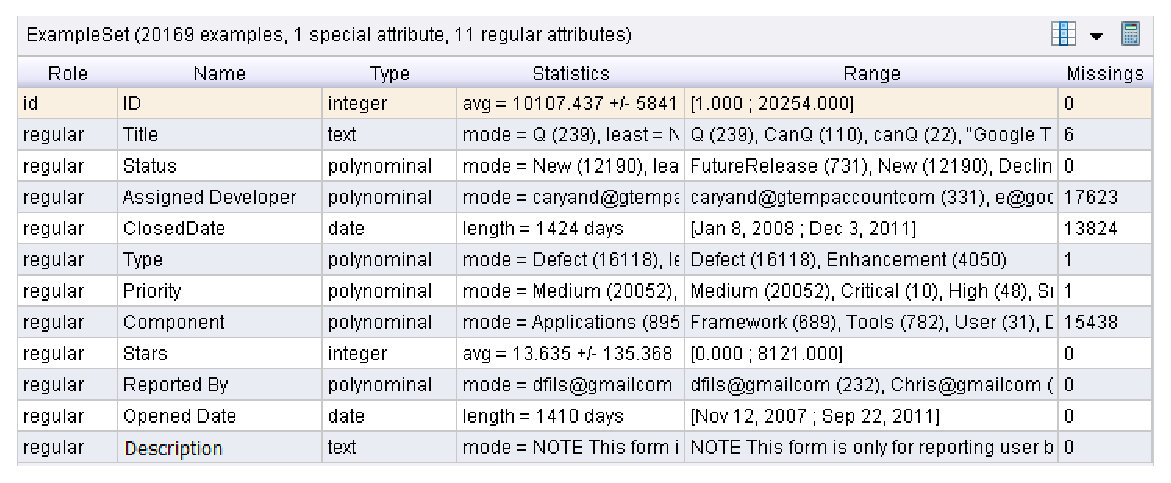
\includegraphics[scale=0.5]{ml3_data_types}
\caption{Defined types for imported data in Rapid Miner}
\end{center}
\end{figure}

Properties of type {\it text} will be later converted to vectors using the text processing features of the data mining software.

